
%% this section contains 33 problems

%% NOTE: do globally
%%------------------------------
%\sisetup{
%    fraction-function = \sfrac,
%}

%% PGFplots Customization
%%------------------------------
\pgfplotsset{
    myaxis/.style={
        axis y line=left,
        axis x line=middle,
        axis line style={->},
        label style={font=\normalsize},
        xtick=\empty,
        x label style={
            at={(current axis.right of origin)},
            anchor=west,
        },
        ytick=\empty,
        y label style={
            at={(current axis.above origin)},
            anchor=south,
            rotate=270,
        },
        width=0.90\columnwidth,
        very thin,
    },
    mystyle/.style={
        line width=1pt,
    },
    mygroup/.style={
        %axis y line=left,
        %axis x line=middle,
        axis lines=middle,
        axis line style={->},
        label style={font=\normalsize},
        xtick=\empty,
        %xmin=0,xmax=10,
        x label style={
            at={(current axis.right of origin)},
            anchor=west,
        },
        %ymin=0,ymax=10,
        ytick=\empty,
        y label style={
            at={(current axis.above origin)},
            anchor=south,
            %rotate=90,
        },
        %x label style={
        %    at={(current axis.right of origin)},
        %    anchor=north east,
        %},
        %y label style={
        %    at={(current axis.above origin)},
        %    anchor=south east,
        %    rotate=90
        %},
        width=0.5\columnwidth,
        height=0.309\columnwidth,
        very thin,
    },
}

%\pgfplotsset{
%    myaxis/.style={
%        axis lines=middle,
%        axis line style={->},
%        x label style={at={(current axis.right of origin)},
%                       anchor=north east},
%        y label style={at={(current axis.above origin)},
%                       anchor=south east,rotate=90},
%        %x label style={at={(0.5,0.0)}},
%        %y label style={at={(0.0,0.5)}}
%        ytick=\empty,
%        xtick=\empty,
%        xlabel={time},
%        ylabel={position},
%        xmin=0,xmax=1,
%        ymin=0,ymax=1,
%        domain=0:2,
%        width=\columnwidth,
%    },
%    mystyle/.style={
%        line width=1pt,
%    }}

%% Custom Graphs
%%--------------------
\newcommand{\myDisplacementGraph}{
    \begin{tikzpicture}
        \begin{axis}[
            myaxis,
            xlabel={$t$},
            x unit=\si{\second},
            ylabel={$x$},
            y unit=\si{\meter},
            xtick={0,4,8,12,16},
            ytick={0,30,60},
            grid=major,
            minor y tick num=1,
            minor x tick num=1,
            xmin=0,xmax=16,
            ymin=0,ymax=70,
            width=0.8\columnwidth,
            height=0.5\columnwidth,
        ]
        \addplot[mystyle,domain=0:6]{10*x};
        \addplot[mystyle,domain=6:10]{60};
        \addplot[mystyle,domain=10:16]{160-10*x};
        \end{axis}
    \end{tikzpicture}
}

\newcommand{\myVelocityGraph}{
    \begin{tikzpicture}
        \begin{axis}[
            myaxis,
            xlabel={$t$},
            x unit=\si{\second},
            ylabel={$v$},
            y unit=\si{\meter\per\second},
            xtick={0,4,8,12,16},
            ytick={0,4,8},
            grid=major,
            minor y tick num=1,
            minor x tick num=1,
            xmin=0,xmax=16,
            ymin=0,ymax=10,
            width=0.8\columnwidth,
            height=0.5\columnwidth,
        ]
        \addplot[mystyle,domain=0:4]{2*x};
        \addplot[mystyle,domain=4:8]{8};
        \addplot[mystyle,domain=8:12]{16-x};
        \addplot[mystyle,domain=12:16]{4};
        \end{axis}
    \end{tikzpicture}
}

\newcommand{\myAccelerationGraph}{
    \begin{tikzpicture}
        \begin{axis}[
            myaxis,
            xlabel={$t$},
            x unit=\si{\second},
            ylabel={$a$},
            y unit=\si{\meter\per\second\squared},
            xtick={0,4,8,12,16},
            ytick={0,4,8},
            grid=major,
            minor y tick num=1,
            minor x tick num=1,
            xmin=0,xmax=16,
            ymin=0,ymax=9,
            width=0.8\columnwidth,
            height=0.5\columnwidth,
        ]
        \addplot[mystyle,domain=0:8]{4};
        \addplot[mystyle,domain=8:16]{8};
        \end{axis}
    \end{tikzpicture}
}

%% Section: Graphing Displacement
%%------------------------------
\element{graphs}{
\begin{question}{graphs-Q01-A}
    Consider the motion of an object whose
        displacement-time graph is provided below.
    \begin{center}
        \myDisplacementGraph
    \end{center}
    What is the instantaneous velocity of the object at
        $t=\SI{4}{\second}$?
    \begin{multicols}{3}
    \begin{choices}
        \wrongchoice{\SI{2}{\meter\per\second}}
        \wrongchoice{\SI{4}{\meter\per\second}}
        \wrongchoice{\SI{8}{\meter\per\second}}
      \correctchoice{\SI{10}{\meter\per\second}}
        \wrongchoice{\SI{20}{\meter\per\second}}
        \wrongchoice{\SI{80}{\meter\per\second}}
    \end{choices}
    \end{multicols}
\end{question}
}

\element{graphs}{
\begin{question}{graphs-Q01-B}
    Consider the motion of an object whose
        displacement-time graph is provided below.
    \begin{center}
        \myDisplacementGraph
    \end{center}
    What is the instantaneous velocity of the object at
        $t=\SI{8}{\second}$?
    \begin{multicols}{3}
    \begin{choices}
      \correctchoice{\SI{0}{\meter\per\second}}
        \wrongchoice{\SI{2}{\meter\per\second}}
        \wrongchoice{\SI{15/2}{\meter\per\second}}
        \wrongchoice{\SI{75/2}{\meter\per\second}}
        \wrongchoice{\SI{60}{\meter\per\second}}
        \wrongchoice{\SI{300}{\meter\per\second}}
    \end{choices}
    \end{multicols}
\end{question}
}

\element{graphs}{
\begin{question}{graphs-Q01-C}
    Consider the motion of an object whose
        displacement-time graph is provided below.
    \begin{center}
        \myDisplacementGraph
    \end{center}
    What is the instantaneous velocity of the object at
        $t=\SI{12}{\second}$?
    \begin{multicols}{3}
    \begin{choices}
      \correctchoice{\SI{-10}{\meter\per\second}}
        \wrongchoice{\SI{10}{\meter\per\second}}
        \wrongchoice{\SI{40}{\meter\per\second}}
        \wrongchoice{\SI{10/3}{\meter\per\second}}
        \wrongchoice{\SI{20/3}{\meter\per\second}}
        \wrongchoice{\SI{80}{\meter\per\second}}
    \end{choices}
    \end{multicols}
\end{question}
}

\element{graphs}{
\begin{question}{graphs-Q01-D}
    Consider the motion of an object whose
        displacement-time graph is provided below.
    \begin{center}
        \myDisplacementGraph
    \end{center}
    What is the average velocity of the object
        between $t=\SI{0}{\second}$ and $t=\SI{4}{\second}$?
    \begin{multicols}{3}
    \begin{choices}
        \wrongchoice{\SI{2}{\meter\per\second}}
        \wrongchoice{\SI{4}{\meter\per\second}}
        \wrongchoice{\SI{8}{\meter\per\second}}
      \correctchoice{\SI{10}{\meter\per\second}}
        \wrongchoice{\SI{20}{\meter\per\second}}
        \wrongchoice{\SI{80}{\meter\per\second}}
    \end{choices}
    \end{multicols}
\end{question}
}

\element{graphs}{
\begin{question}{graphs-Q01-E}
    Consider the motion of an object whose
        displacement-time graph is provided below.
    \begin{center}
        \myDisplacementGraph
    \end{center}
    What is the average velocity of the object
        between $t=\SI{0}{\second}$ and $t=\SI{8}{\second}$?
    \begin{multicols}{3}
    \begin{choices}
        \wrongchoice{\SI{0}{\meter\per\second}}
        \wrongchoice{\SI{2}{\meter\per\second}}
      \correctchoice{\SI{15/2}{\meter\per\second}}
        \wrongchoice{\SI{75/2}{\meter\per\second}}
        \wrongchoice{\SI{60}{\meter\per\second}}
        \wrongchoice{\SI{300}{\meter\per\second}}
    \end{choices}
    \end{multicols}
\end{question}
}

\element{graphs}{
\begin{question}{graphs-Q01-F}
    Consider the motion of an object whose
        displacement-time graph is provided below.
    \begin{center}
        \myDisplacementGraph
    \end{center}
    What is the average velocity of the object
        between $t=\SI{0}{\second}$ and $t=\SI{12}{\second}$?
    \begin{multicols}{3}
    \begin{choices}
        \wrongchoice{\SI{-10}{\meter\per\second}}
        \wrongchoice{\SI{10}{\meter\per\second}}
        \wrongchoice{\SI{40}{\meter\per\second}}
      \correctchoice{\SI{10/3}{\meter\per\second}}
        \wrongchoice{\SI{20/3}{\meter\per\second}}
        \wrongchoice{\SI{80}{\meter\per\second}}
    \end{choices}
    \end{multicols}
\end{question}
}

%% Section: Graphing Velocity
%%------------------------------
\element{graphs}{
\begin{question}{graphs-Q02-A}
    Consider the motion of an object whose
        velocity-time graph is provided below.
    \begin{center}
        \myVelocityGraph
    \end{center}
    What is the acceleration of the object at
        $t=\SI{2}{\second}$?
    \begin{multicols}{3}
    \begin{choices}
        \wrongchoice{\SI{-1}{\meter\per\second\squared}}
        \wrongchoice{\SI{0}{\meter\per\second\squared}}
      \correctchoice{\SI{2}{\meter\per\second\squared}}
        \wrongchoice{\SI{4}{\meter\per\second\squared}}
        \wrongchoice{\SI{8}{\meter\per\second\squared}}
        \wrongchoice{\SI{10}{\meter\per\second\squared}}
    \end{choices}
    \end{multicols}
\end{question}
}

\element{graphs}{
\begin{question}{graphs-Q02-B}
    Consider the motion of an object whose
        velocity-time graph is provided below.
    \begin{center}
        \myVelocityGraph
    \end{center}
    What is the acceleration of the object at
        $t=\SI{6}{\second}$?
    \begin{multicols}{3}
    \begin{choices}
        \wrongchoice{\SI{-1}{\meter\per\second\squared}}
      \correctchoice{\SI{0}{\meter\per\second\squared}}
        \wrongchoice{\SI{2}{\meter\per\second\squared}}
        \wrongchoice{\SI{4}{\meter\per\second\squared}}
        \wrongchoice{\SI{8}{\meter\per\second\squared}}
        \wrongchoice{\SI{10}{\meter\per\second\squared}}
    \end{choices}
    \end{multicols}
\end{question}
}

\element{graphs}{
\begin{question}{graphs-Q02-C}
    Consider the motion of an object whose
        velocity-time graph is provided below.
    \begin{center}
        \myVelocityGraph
    \end{center}
    What is the acceleration of the object at
        $t=\SI{10}{\second}$?
    \begin{multicols}{3}
    \begin{choices}
        \wrongchoice{\SI{-2}{\meter\per\second\squared}}
      \correctchoice{\SI{-1}{\meter\per\second\squared}}
        \wrongchoice{\SI{0}{\meter\per\second\squared}}
        \wrongchoice{\SI{2}{\meter\per\second\squared}}
        \wrongchoice{\SI{4}{\meter\per\second\squared}}
        \wrongchoice{\SI{8}{\meter\per\second\squared}}
    \end{choices}
    \end{multicols}
\end{question}
}

\element{graphs}{
\begin{question}{graphs-Q02-D}
    Consider the motion of an object whose
        velocity-time graph is provided below.
    \begin{center}
        \myVelocityGraph
    \end{center}
    What is the acceleration of the object at
        $t=\SI{14}{\second}$?
    \begin{multicols}{3}
    \begin{choices}
        \wrongchoice{\SI{-1}{\meter\per\second\squared}}
      \correctchoice{\SI{0}{\meter\per\second\squared}}
        \wrongchoice{\SI{2}{\meter\per\second\squared}}
        \wrongchoice{\SI{4}{\meter\per\second\squared}}
        \wrongchoice{\SI{8}{\meter\per\second\squared}}
        \wrongchoice{\SI{10}{\meter\per\second\squared}}
    \end{choices}
    \end{multicols}
\end{question}
}

\element{graphs}{
\begin{question}{graphs-Q02-E}
    Consider the motion of an object whose
        velocity-time graph is provided below.
    \begin{center}
        \myVelocityGraph
    \end{center}
    What is the displacement of the object between
        $t=\SI{0}{\second}$ and $t=\SI{10}{\second}$?
    \begin{multicols}{3}
    \begin{choices}
        \wrongchoice{\SI{6}{\meter}}
        \wrongchoice{\SI{-1}{\meter}}
        \wrongchoice{\SI{0.6}{\meter}}
      \correctchoice{\SI{62}{\meter}}
        \wrongchoice{\SI{72}{\meter}}
        \wrongchoice{\SI{88}{\meter}}
    \end{choices}
    \end{multicols}
\end{question}
}

\element{graphs}{
\begin{question}{graphs-Q02-F}
    Consider the motion of an object whose
        velocity-time graph is provided below.
    \begin{center}
        \myVelocityGraph
    \end{center}
    What is the displacement of the object between
        $t=\SI{0}{\second}$ and $t=\SI{14}{\second}$?
    \begin{multicols}{3}
    \begin{choices}
        \wrongchoice{\SI{0}{\meter}}
        \wrongchoice{\SI{2/7}{\meter}}
        \wrongchoice{\SI{4}{\meter}}
        \wrongchoice{\SI{72}{\meter}}
      \correctchoice{\SI{80}{\meter}}
        \wrongchoice{\SI{88}{\meter}}
    \end{choices}
    \end{multicols}
\end{question}
}

\element{graphs}{
\begin{question}{graphs-Q02-G}
    Consider the motion of an object whose
        velocity-time graph is provided below.
    \begin{center}
        \myVelocityGraph
    \end{center}
    What is the average velocity between
        $t=\SI{0}{\second}$ and $t=\SI{10}{\second}$?
    \begin{multicols}{3}
    \begin{choices}
        \wrongchoice{\SI{-1}{\meter\per\second}}
        \wrongchoice{\SI{6}{\meter\per\second}}
        \wrongchoice{\SI{3/5}{\meter\per\second}}
        \wrongchoice{\SI{24/5}{\meter\per\second}}
      \correctchoice{\SI{31/5}{\meter\per\second}}
        \wrongchoice{\SI{36/5}{\meter\per\second}}
    \end{choices}
    \end{multicols}
\end{question}
}

\element{graphs}{
\begin{question}{graphs-Q02-H}
    Consider the motion of an object whose
        velocity-time graph is provided below.
    \begin{center}
        \myVelocityGraph
    \end{center}
    What is the average velocity between
        $t=\SI{0}{\second}$ and $t=\SI{14}{\second}$?
    \begin{multicols}{3}
    \begin{choices}
        \wrongchoice{\SI{4}{\meter\per\second}}
        \wrongchoice{\SI{0}{\meter\per\second}}
        \wrongchoice{\SI{2}{\meter\per\second}}
        \wrongchoice{\SI{36/7}{\meter\per\second}}
      \correctchoice{\SI{40/7}{\meter\per\second}}
        \wrongchoice{\SI{11/2}{\meter\per\second}}
    \end{choices}
    \end{multicols}
\end{question}
}


%% Section: Graphing Acceleration
%%------------------------------
\element{graphs}{
\begin{question}{graphs-Q03-A}
    Consider the motion of an object that starts from rest
        and whose acceleration-time graph is provided below.
    \begin{center}
        \myAccelerationGraph
    \end{center}
    What is the average velocity between
        $t=\SI{0}{\second}$ and $t=\SI{8}{\second}$?
    \begin{multicols}{3}
    \begin{choices}
        \wrongchoice{\SI{0}{\meter\per\second}}
        \wrongchoice{\SI{2}{\meter\per\second}}
        \wrongchoice{\SI{4}{\meter\per\second}}
      \correctchoice{\SI{16}{\meter\per\second}}
        \wrongchoice{\SI{32}{\meter\per\second}}
        \wrongchoice{\SI{64}{\meter\per\second}}
    \end{choices}
    \end{multicols}
\end{question}
}

\element{graphs}{
\begin{question}{graphs-Q03-B}
    Consider the motion of an object that starts from rest
        and whose acceleration-time graph is provided below.
    \begin{center}
        \myAccelerationGraph
    \end{center}
    What is the average velocity between
        $t=\SI{0}{\second}$ and $t=\SI{16}{\second}$?
    \begin{multicols}{3}
    \begin{choices}
        \wrongchoice{\SI{16}{\meter\per\second}}
        \wrongchoice{\SI{32}{\meter\per\second}}
      \correctchoice{\SI{40}{\meter\per\second}}
        \wrongchoice{\SI{64}{\meter\per\second}}
        \wrongchoice{\SI{96}{\meter\per\second}}
        \wrongchoice{\SI{128}{\meter\per\second}}
    \end{choices}
    \end{multicols}
\end{question}
}

\element{graphs}{
\begin{question}{graphs-Q03-C}
    Consider the motion of an object that starts from rest
        and whose acceleration-time graph is provided below.
    \begin{center}
        \myAccelerationGraph
    \end{center}
    What is the total displacement between
        $t=\SI{0}{\second}$ and $t=\SI{8}{\second}$?
    \begin{multicols}{3}
    \begin{choices}
        \wrongchoice{\SI{0}{\meter}}
        \wrongchoice{\SI{4}{\meter}}
        \wrongchoice{\SI{16}{\meter}}
        \wrongchoice{\SI{32}{\meter}}
      \correctchoice{\SI{128}{\meter}}
        \wrongchoice{\SI{11/2}{\meter}}
    \end{choices}
    \end{multicols}
\end{question}
}

\element{graphs}{
\begin{question}{graphs-Q03-D}
    Consider the motion of an object that starts from rest
        and whose acceleration-time graph is provided below.
    \begin{center}
        \myAccelerationGraph
    \end{center}
    What is the total displacement between
        $t=\SI{0}{\second}$ and $t=\SI{16}{\second}$?
    \begin{multicols}{3}
    \begin{choices}
        \wrongchoice{\SI{96}{\meter}}
        \wrongchoice{\SI{160}{\meter}}
        \wrongchoice{\SI{256}{\meter}}
        \wrongchoice{\SI{512}{\meter}}
      \correctchoice{\SI{640}{\meter}}
        \wrongchoice{\SI{1024}{\meter}}
    \end{choices}
    \end{multicols}
\end{question}
}

%\element{graphs}{
%\begin{question}{graphs-Q03-E}
%    Consider the motion of an object that starts from rest
%       and whose acceleration-time graph is provided below.
%    \begin{center}
%        \myAccelerationGraph
%    \end{center}
%    What is the instantaneous velocity of the object at
%        $t=\SI{4}{\second}$?
%    \begin{multicols}{3}
%    \begin{choices}
%        \wrongchoice{\SI{0}{\meter\per\second}}
%    \end{choices}
%    \end{multicols}
%\end{question}
%}

%\element{graphs}{
%\begin{question}{graphs-Q03-F}
%    Consider the motion of an object that starts from rest
%       and whose acceleration-time graph is provided below.
%    \begin{center}
%        \myAccelerationGraph
%    \end{center}
%    What is the instantaneous velocity of the object at
%        $t=\SI{12}{\second}$?
%    \begin{multicols}{3}
%    \begin{choices}
%        \wrongchoice{\SI{0}{\meter\per\second}}
%    \end{choices}
%    \end{multicols}
%\end{question}
%}


%% Section: Descriptive graphs
%%------------------------------
\element{graphs}{
\begin{question}{graphs-Q11}
    Consider the motion of an object whose motion is shown in the diagram below.
    \begin{center}
    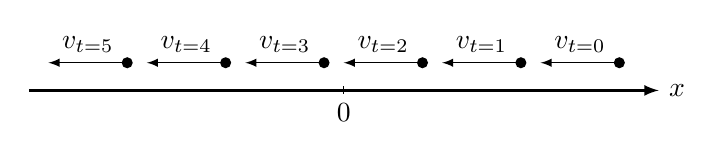
\begin{tikzpicture}
        \draw[thick,-latex] (-4,0) -- (4,0) node[anchor=west] {$x$};
        \draw (0,0.05) -- (0,-0.05) node[anchor=north] {$0$};
        \foreach \x in {0,1,...,5} {
            \fill ({3.5-1.25*\x},1em) circle (2pt);
            \draw[-latex] ({3.5-1.25*\x},1em) -- ++(180:1) node[pos=0.5,anchor=south] {$v_{t=\x}$};
        }
    \end{tikzpicture}
    \end{center}
    Which displacement-time graph best represents the motion shown in the diagram?
    \begin{multicols}{2}
    \begin{choices}
        \AMCboxDimensions{down=-2.5em}
        \wrongchoice{
            \begin{tikzpicture}
                \begin{axis}[
                    myaxis,
                    xlabel={$t$},
                    ylabel={$x$},
                    xtick=\empty,
                    ytick=\empty,
                    xmin=0,xmax=10,
                    ymin=-10,ymax=10,
                    width=\columnwidth,
                ]
                \addplot[mystyle,domain=0:10]{2 + 0.8*x};
                \end{axis}
            \end{tikzpicture}
        }
        \wrongchoice{
            \begin{tikzpicture}
                \begin{axis}[
                    myaxis,
                    xlabel={$t$},
                    ylabel={$x$},
                    xtick=\empty,
                    ytick=\empty,
                    xmin=0,xmax=10,
                    ymin=-10,ymax=10,
                    width=\columnwidth,
                ]
                \addplot[mystyle,domain=0:10]{0.8*x};
                \end{axis}
            \end{tikzpicture}
        }
        \wrongchoice{
            \begin{tikzpicture}
                \begin{axis}[
                    myaxis,
                    xlabel={$t$},
                    ylabel={$x$},
                    xtick=\empty,
                    ytick=\empty,
                    xmin=0,xmax=10,
                    ymin=-10,ymax=10,
                    width=\columnwidth,
                ]
                \addplot[mystyle,domain=0:10]{4};
                \end{axis}
            \end{tikzpicture}
        }
        \correctchoice{
            \begin{tikzpicture}
                \begin{axis}[
                    myaxis,
                    xlabel={$t$},
                    ylabel={$x$},
                    xtick=\empty,
                    ytick=\empty,
                    xmin=0,xmax=10,
                    ymin=-10,ymax=10,
                    width=\columnwidth,
                ]
                \addplot[mystyle,domain=0:10]{6 - 1.2*x};
                \end{axis}
            \end{tikzpicture}
        }
        \wrongchoice{
            \begin{tikzpicture}
                \begin{axis}[
                    myaxis,
                    xlabel={$t$},
                    ylabel={$x$},
                    xtick=\empty,
                    ytick=\empty,
                    xmin=0,xmax=10,
                    ymin=-10,ymax=10,
                    width=\columnwidth,
                ]
                \addplot[mystyle,domain=0:10]{-0.8*x};
                \end{axis}
            \end{tikzpicture}
        }
        \wrongchoice{
            \begin{tikzpicture}
                \begin{axis}[
                    myaxis,
                    xlabel={$t$},
                    ylabel={$x$},
                    xtick=\empty,
                    ytick=\empty,
                    xmin=0,xmax=10,
                    ymin=-10,ymax=10,
                    width=\columnwidth,
                ]
                \addplot[mystyle,domain=0:10]{-2 - 0.8*x};
                \end{axis}
            \end{tikzpicture}
        }
    \end{choices}
    \end{multicols}
\end{question}
}


\element{graphs}{
\begin{question}{graphs-Q12}
    Which velocity-time graph best describes the
        motion shown in the displacement-time graph below?
    \begin{center}
    \begin{tikzpicture}
        \begin{axis}[
            myaxis,
            xlabel={$t$},
            ylabel={$x$},
            xtick=\empty,
            ytick=\empty,
            xmin=0,xmax=10,
            ymin=-10,ymax=10,
            width=0.8\columnwidth,
            height=0.50\columnwidth,
        ]
        \addplot[mystyle,domain=0:4]{-8 + 2*x};
        \addplot[mystyle,domain=4:10]{2*(x-4) - (2/12) * (x-4)^2};
        \end{axis}
    \end{tikzpicture}
    \end{center}
    \begin{multicols}{2}
    \begin{choices}
        \AMCboxDimensions{down=-2.5em}
        \correctchoice{
            \begin{tikzpicture}
                \begin{axis}[
                    myaxis,
                    xlabel={$t$},
                    ylabel={$v$},
                    xtick=\empty,
                    ytick=\empty,
                    xmin=0,xmax=10,
                    ymin=-10,ymax=10,
                    width=\columnwidth,
                    %height=0.618\columnwidth,
                ]
                \addplot[mystyle,domain=0:4]{8};
                \addplot[mystyle,domain=4:10]{(40/3) - (4/3)*x};
                \end{axis}
            \end{tikzpicture}
        }
        \wrongchoice{
            \begin{tikzpicture}
                \begin{axis}[
                    myaxis,
                    xlabel={$t$},
                    ylabel={$v$},
                    xtick=\empty,
                    ytick=\empty,
                    xmin=0,xmax=10,
                    ymin=-10,ymax=10,
                    width=\columnwidth,
                    %height=0.618\columnwidth,
                ]
                \addplot[mystyle,domain=0:4]{-8};
                \addplot[mystyle,domain=4:10]{-(40/3) + (4/3)*x};
                \end{axis}
            \end{tikzpicture}
        }
        \wrongchoice{
            \begin{tikzpicture}
                \begin{axis}[
                    myaxis,
                    xlabel={$t$},
                    ylabel={$v$},
                    xtick=\empty,
                    ytick=\empty,
                    xmin=0,xmax=10,
                    ymin=-10,ymax=10,
                    width=\columnwidth,
                    %height=0.618\columnwidth,
                ]
                \addplot[mystyle,domain=0:4]{-8 + 2*x};
                \addplot[mystyle,domain=4:10]{2*(x-4) - (2/12)*(x-4)^2};
                \end{axis}
            \end{tikzpicture}
        }
        \wrongchoice{
            \begin{tikzpicture}
                \begin{axis}[
                    myaxis,
                    xlabel={$t$},
                    ylabel={$v$},
                    xtick=\empty,
                    ytick=\empty,
                    xmin=0,xmax=10,
                    ymin=-10,ymax=10,
                    width=\columnwidth,
                    %height=0.618\columnwidth,
                ]
                \addplot[mystyle,domain=0:4]{8 - 2*x};
                \addplot[mystyle,domain=4:10]{-2*(x-4) + (2/12)*(x-4)^2};
                \end{axis}
            \end{tikzpicture}
        }
        \wrongchoice{
            \begin{tikzpicture}
                \begin{axis}[
                    myaxis,
                    xlabel={$t$},
                    ylabel={$v$},
                    xtick=\empty,
                    ytick=\empty,
                    xmin=0,xmax=10,
                    ymin=-10,ymax=10,
                    width=\columnwidth,
                    %height=0.618\columnwidth,
                ]
                \addplot[mystyle,domain=0:4]{-4 + 0.25 * x^2};
                \addplot[mystyle,domain=4:10]{2*(x-4)};
                \end{axis}
            \end{tikzpicture}
        }
        \wrongchoice{
            \begin{tikzpicture}
                \begin{axis}[
                    myaxis,
                    xlabel={$t$},
                    ylabel={$v$},
                    xtick=\empty,
                    ytick=\empty,
                    xmin=0,xmax=10,
                    ymin=-10,ymax=10,
                    width=\columnwidth,
                    %height=0.618\columnwidth,
                ]
                \addplot[mystyle,domain=0:4]{4 - 0.25 *x^2};
                \addplot[mystyle,domain=4:10]{-2*(x-4)};
                \end{axis}
            \end{tikzpicture}
        }
    \end{choices}
    \end{multicols}
\end{question}
}

\element{graphs}{
\begin{question}{graphs-Q13}
    Which velocity-time graph best describes the
        motion shown in the displacement-time graph below?
    \begin{center}
    \begin{tikzpicture}
        \begin{axis}[
            myaxis,
            xlabel={$t$},
            ylabel={$x$},
            xtick=\empty,
            ytick=\empty,
            xmin=0,xmax=12,
            ymin=0,ymax=20,
            width=0.8\columnwidth,
            height=0.5\columnwidth,
        ]
        \addplot[mystyle,domain=0:4]{0.25 * x^2};
        \addplot[mystyle,domain=4:8,dashed]{4 + 2*(x-4)};
        \addplot[mystyle,domain=8:12]{-20 + 6*x - 0.25*x^2};
        \end{axis}
    \end{tikzpicture}
    \end{center}
    The middle section is dashed to emphasize
        the transition in the curve.
    \begin{multicols}{2}
    \begin{choices}
        \AMCboxDimensions{down=-2.5em}
        \correctchoice{
            \begin{tikzpicture}
                \begin{axis}[
                    myaxis,
                    xlabel={$t$},
                    ylabel={$v$},
                    xtick=\empty,
                    ytick=\empty,
                    xmin=0,xmax=12,
                    ymin=0,ymax=5,
                    width=\columnwidth,
                    %height=0.618\columnwidth,
                ]
                \addplot[mystyle,domain=0:4]{0.5 * x};
                \addplot[mystyle,domain=4:8]{2};
                \addplot[mystyle,domain=8:12]{2 - 0.5*(x-8)};
                \end{axis}
            \end{tikzpicture}
        }
        \wrongchoice{
            \begin{tikzpicture}
                \begin{axis}[
                    myaxis,
                    xlabel={$t$},
                    ylabel={$v$},
                    xtick=\empty,
                    ytick=\empty,
                    xmin=0,xmax=12,
                    ymin=0,ymax=5,
                    width=\columnwidth,
                    %height=0.618\columnwidth,
                ]
                \addplot[mystyle,domain=0:4]{5 - 0.5 *x};
                \addplot[mystyle,domain=4:8]{3};
                \addplot[mystyle,domain=8:12]{3 - 0.5*(x-8)};
                \end{axis}
            \end{tikzpicture}
        }
        \wrongchoice{
            \begin{tikzpicture}
                \begin{axis}[
                    myaxis,
                    xlabel={$t$},
                    ylabel={$v$},
                    xtick=\empty,
                    ytick=\empty,
                    xmin=0,xmax=12,
                    ymin=0,ymax=5,
                    width=\columnwidth,
                    %height=0.618\columnwidth,
                ]
                \addplot[mystyle,domain=0:4]{1};
                \addplot[mystyle,domain=4:8]{1 + 0.75*(x-4)};
                \addplot[mystyle,domain=8:12]{4};
                \end{axis}
            \end{tikzpicture}
        }
        \wrongchoice{
            \begin{tikzpicture}
                \begin{axis}[
                    myaxis,
                    xlabel={$t$},
                    ylabel={$v$},
                    xtick=\empty,
                    ytick=\empty,
                    xmin=0,xmax=12,
                    ymin=0,ymax=5,
                    width=\columnwidth,
                    %height=0.618\columnwidth,
                ]
                \addplot[mystyle,domain=0:4]{4};
                \addplot[mystyle,domain=4:8]{4 - 0.75*(x-4)};
                \addplot[mystyle,domain=8:12]{1};
                \end{axis}
            \end{tikzpicture}
        }
        \wrongchoice{
            \begin{tikzpicture}
                \begin{axis}[
                    myaxis,
                    xlabel={$t$},
                    ylabel={$v$},
                    xtick=\empty,
                    ytick=\empty,
                    xmin=0,xmax=12,
                    ymin=0,ymax=5,
                    width=\columnwidth,
                    %height=0.618\columnwidth,
                ]
                \addplot[mystyle,domain=0:4]{0.5 * x};
                \addplot[mystyle,domain=4:8]{2};
                \addplot[mystyle,domain=8:12]{2 + 0.5*(x-8)};
                \end{axis}
            \end{tikzpicture}
        }
        \wrongchoice{
            \begin{tikzpicture}
                \begin{axis}[
                    myaxis,
                    xlabel={$t$},
                    ylabel={$v$},
                    xtick=\empty,
                    ytick=\empty,
                    xmin=0,xmax=12,
                    ymin=0,ymax=5,
                    width=\columnwidth,
                    %height=0.618\columnwidth,
                ]
                \addplot[mystyle,domain=0:4]{0.125 * x};
                \addplot[mystyle,domain=4:8]{0.5 + 0.75*(x-4)};
                \addplot[mystyle,domain=8:12]{3.5 + 0.125*(x-8)};
                \end{axis}
            \end{tikzpicture}
        }
    \end{choices}
    \end{multicols}
\end{question}
}

\element{graphs}{
\begin{question}{graphs-Q14}
    Which displacement-time graph best describes the
        motion shown in the velocity-time graph below?
    \begin{center}
    \begin{tikzpicture}
        \begin{axis}[
            myaxis,
            xlabel={$t$},
            x unit=\si{\meter},
            xmin=0,xmax=11,
            ylabel={$v$},
            y unit=\si{\meter\per\second},
            ymin=-3,ymax=5,
            xtick={0,5,10},
            ytick={-2,0,2,4},
            minor y tick num=1,
            minor x tick num=1,
            width=0.8\columnwidth,
            height=0.5\columnwidth,
        ]
        \addplot[mystyle,domain=0:5]{4};
        \addplot[mystyle,domain=5:10]{-2};
        \addplot[mystyle,dashed,mark=\empty]
            plot coordinates{ (5,4) (5,-2) };
        \end{axis}
    \end{tikzpicture}
    \end{center}
    The particle's position at $t_i=\SI{0}{\second}$ is
        $x_i=\SI{-10}{\meter}$.
    \begin{multicols}{2}
    \begin{choices}
        \AMCboxDimensions{down=-2.30em}
        \correctchoice{
            \hspace{-1.85em}
            \begin{tikzpicture}
                \begin{axis}[
                    myaxis,
                    xlabel={$t$},
                    x unit=\si{\second},
                    xmin=0,xmax=11,
                    ylabel={$x$},
                    y unit=\si{\meter},
                    ymin=-11,ymax=11,
                    xtick={0,5,10},
                    ytick={-10,0,10},
                    minor y tick num=1,
                    minor x tick num=1,
                    width=0.95\columnwidth,
                ]
                \addplot[mystyle,domain=0:5]{-10+4*x};
                \addplot[mystyle,domain=5:10]{20-2*x};
                \end{axis}
            \end{tikzpicture}
        }
        \wrongchoice{
            \hspace{-1.85em}
            \begin{tikzpicture}
                \begin{axis}[
                    myaxis,
                    xlabel={$t$},
                    x unit=\si{\second},
                    xmin=0,xmax=11,
                    ylabel={$x$},
                    y unit=\si{\meter},
                    ymin=-11,ymax=11,
                    xtick={0,5,10},
                    ytick={-10,0,10},
                    minor y tick num=1,
                    minor x tick num=1,
                    width=0.95\columnwidth,
                ]
                \addplot[mystyle,domain=0:5]{-10};
                \addplot[mystyle,domain=5:10]{5};
                \addplot[mystyle,dashed,mark=\empty]
                    plot coordinates{ (5,-10) (5,5) };
                \end{axis}
            \end{tikzpicture}
        }
        \wrongchoice{
            \hspace{-1.85em}
            \begin{tikzpicture}
                \begin{axis}[
                    myaxis,
                    xlabel={$t$},
                    x unit=\si{\second},
                    xmin=0,xmax=11,
                    ylabel={$x$},
                    y unit=\si{\meter},
                    ymin=-11,ymax=11,
                    xtick={0,5,10},
                    ytick={-10,0,10},
                    minor y tick num=1,
                    minor x tick num=1,
                    width=0.95\columnwidth,
                ]
                \addplot[mystyle,domain=0:5]{5};
                \addplot[mystyle,domain=5:10]{-2};
                \addplot[mystyle,dashed,mark=\empty]
                    plot coordinates{ (5,5) (5,-2) };
                \end{axis}
            \end{tikzpicture}
        }
        \wrongchoice{
            \hspace{-1.85em}
            \begin{tikzpicture}
                \begin{axis}[
                    myaxis,
                    xlabel={$t$},
                    x unit=\si{\second},
                    xmin=0,xmax=11,
                    ylabel={$x$},
                    y unit=\si{\meter},
                    ymin=-11,ymax=11,
                    xtick={0,5,10},
                    ytick={-10,0,10},
                    minor y tick num=1,
                    minor x tick num=1,
                    width=0.95\columnwidth,
                ]
                \addplot[mystyle,domain=0:10]{-10+2*x};
                \end{axis}
            \end{tikzpicture}
        }
    \end{choices}
    \end{multicols}
\end{question}
}

\element{graphs}{
\begin{question}{graphs-Q15}
    Which velocity-time graph best describes the
        motion shown in the acceleration-time graph below?
    The particle is initially moving to the right
        and eventually to the left.
    \begin{center}
    \begin{tikzpicture}
        \begin{axis}[
            myaxis,
            xtick=\empty,
            ytick=\empty,
            xlabel={$t$},
            ylabel={$a$},
            xmin=0,xmax=12,
            ymin=-8,ymax=8,
            width=0.8\columnwidth,
            height=0.5\columnwidth,
        ]
        \addplot[mystyle,domain=0:4]{0};
        \addplot[mystyle,domain=4:8]{-4};
        \addplot[mystyle,domain=8:12]{0};
        \addplot[mystyle,dashed,mark=\empty]
            plot coordinates{ (4,0) (4,-4) };
        \addplot[mystyle,dashed,mark=\empty]
            plot coordinates{ (8,0) (8,-4) };
        \end{axis}
    \end{tikzpicture}
    \end{center}
    \begin{multicols}{2}
    \begin{choices}
        \AMCboxDimensions{down=-2em}
        \correctchoice{
            \begin{tikzpicture}
                \begin{axis}[
                    myaxis,
                    xtick=\empty,
                    ytick=\empty,
                    xlabel={$t$},
                    ylabel={$v$},
                    ymin=-13,ymax=13,
                    xmin=0,xmax=13,
                    width=\columnwidth,
                ]
                \addplot[mystyle,domain=0:4]{4};
                \addplot[mystyle,domain=4:8]{12-2*x};
                \addplot[mystyle,domain=8:12]{-4};
                \end{axis}
            \end{tikzpicture}
        }
        \wrongchoice{
            \begin{tikzpicture}
                \begin{axis}[
                    myaxis,
                    xtick=\empty,
                    ytick=\empty,
                    xlabel={$t$},
                    ylabel={$v$},
                    ymin=-13,ymax=13,
                    xmin=0,xmax=13,
                    width=\columnwidth,
                ]
                \addplot[mystyle,domain=0:4]{10};
                \addplot[mystyle,domain=4:8]{18-2*x};
                \addplot[mystyle,domain=8:12]{2};
                \end{axis}
            \end{tikzpicture}
        }
        \wrongchoice{
            \begin{tikzpicture}
                \begin{axis}[
                    myaxis,
                    xtick=\empty,
                    ytick=\empty,
                    xlabel={$t$},
                    ylabel={$v$},
                    ymin=-13,ymax=13,
                    xmin=0,xmax=13,
                    width=\columnwidth,
                ]
                \addplot[mystyle,domain=0:4]{-2};
                \addplot[mystyle,domain=4:8]{6-2*x};
                \addplot[mystyle,domain=8:12]{-10};
                \end{axis}
            \end{tikzpicture}
        }
        \wrongchoice{
            \begin{tikzpicture}
                \begin{axis}[
                    myaxis,
                    xtick=\empty,
                    ytick=\empty,
                    xlabel={$t$},
                    ylabel={$v$},
                    ymin=-13,ymax=13,
                    xmin=0,xmax=13,
                    width=\columnwidth,
                ]
                \addplot[mystyle,domain=0:4]{12};
                \addplot[mystyle,domain=4:8]{0};
                \addplot[mystyle,domain=8:12]{12};
                \addplot[mystyle,dashed,mark=\empty]
                    plot coordinates{ (4,12) (4,0) };
                \addplot[mystyle,dashed,mark=\empty]
                    plot coordinates{ (8,12) (8,0) };
                \end{axis}
            \end{tikzpicture}
        }
        \wrongchoice{
            \begin{tikzpicture}
                \begin{axis}[
                    myaxis,
                    xtick=\empty,
                    ytick=\empty,
                    xlabel={$t$},
                    ylabel={$v$},
                    ymin=-13,ymax=13,
                    xmin=0,xmax=13,
                    width=\columnwidth,
                ]
                \addplot[mystyle,domain=0:4]{-12};
                \addplot[mystyle,domain=4:8]{0};
                \addplot[mystyle,domain=8:12]{-12};
                \addplot[mystyle,dashed,mark=\empty]
                    plot coordinates{ (4,-12) (4,0) };
                \addplot[mystyle,dashed,mark=\empty]
                    plot coordinates{ (8,-12) (8,0) };
                \end{axis}
            \end{tikzpicture}
        }
        \wrongchoice{
            \begin{tikzpicture}
                \begin{axis}[
                    myaxis,
                    xtick=\empty,
                    ytick=\empty,
                    xlabel={$t$},
                    ylabel={$v$},
                    ymin=-13,ymax=13,
                    xmin=0,xmax=13,
                    width=\columnwidth,
                ]
                \addplot[mystyle,domain=0:4]{0};
                \addplot[mystyle,domain=4:8]{-12};
                \addplot[mystyle,domain=8:12]{0};
                \addplot[mystyle,dashed,mark=\empty]
                    plot coordinates{ (4,0) (4,-12) };
                \addplot[mystyle,dashed,mark=\empty]
                    plot coordinates{ (8,0) (8,-12) };
                \end{axis}
            \end{tikzpicture}
        }
    \end{choices}
    \end{multicols}
\end{question}
}

\element{graphs}{
\begin{question}{graphs-Q16}
    A ball rolls up a ramp,
        then back down under the influence of gravity.
    Which acceleration-time graph best represents the balls motion?
    Motion up the ramp is defined to be positive.
    \begin{multicols}{2}
    \begin{choices}
        \AMCboxDimensions{down=-2.5em}
        \correctchoice{
            \begin{tikzpicture}
                \begin{axis}[
                    myaxis,
                    xtick=\empty,
                    ytick=\empty,
                    xlabel={$t$},
                    ylabel={$a$},
                    ymin=-10,ymax=10,
                    xmin=0,xmax=10,
                    width=\columnwidth,
                ]
                \addplot[mystyle,domain=0:10]{-8};
                \end{axis}
            \end{tikzpicture}
        }
        \wrongchoice{
            \begin{tikzpicture}
                \begin{axis}[
                    myaxis,
                    xtick=\empty,
                    ytick=\empty,
                    xlabel={$t$},
                    ylabel={$a$},
                    ymin=-10,ymax=10,
                    xmin=0,xmax=10,
                    width=\columnwidth,
                ]
                \addplot[mystyle,domain=0:10]{8-2*x};
                \end{axis}
            \end{tikzpicture}
        }
        \wrongchoice{
            \begin{tikzpicture}
                \begin{axis}[
                    myaxis,
                    xtick=\empty,
                    ytick=\empty,
                    xlabel={$t$},
                    ylabel={$a$},
                    ymin=-10,ymax=10,
                    xmin=0,xmax=10,
                    width=\columnwidth,
                ]
                \addplot[mystyle,domain=0:5]{-8};
                \addplot[mystyle,domain=5:10]{8};
                \addplot[mystyle,dashed,mark=\empty]
                    plot coordinates{ (5,-8) (5,8) };
                \end{axis}
            \end{tikzpicture}
        }
        \wrongchoice{
            \begin{tikzpicture}
                \begin{axis}[
                    myaxis,
                    xtick=\empty,
                    ytick=\empty,
                    xlabel={$t$},
                    ylabel={$a$},
                    ymin=-10,ymax=10,
                    xmin=0,xmax=10,
                    width=\columnwidth,
                ]
                \addplot[mystyle,domain=0:10]{8};
                \end{axis}
            \end{tikzpicture}
        }
        \wrongchoice{
            \begin{tikzpicture}
                \begin{axis}[
                    myaxis,
                    xtick=\empty,
                    ytick=\empty,
                    xlabel={$t$},
                    ylabel={$a$},
                    ymin=-10,ymax=10,
                    xmin=0,xmax=10,
                    width=\columnwidth,
                ]
                \addplot[mystyle,domain=0:4.5]{-8};
                \addplot[mystyle,domain=4.5:5.5]{0};
                \addplot[mystyle,domain=5.5:10]{-8};
                \addplot[mystyle,dashed,mark=\empty]
                    plot coordinates{ (5.5,0) (5.5,-8) };
                \addplot[mystyle,dashed,mark=\empty]
                    plot coordinates{ (4.5,0) (4.5,-8) };
                \end{axis}
            \end{tikzpicture}
        }
        \wrongchoice{
            \begin{tikzpicture}
                \begin{axis}[
                    myaxis,
                    xtick=\empty,
                    ytick=\empty,
                    xlabel={$t$},
                    ylabel={$a$},
                    ymin=-10,ymax=10,
                    xmin=0,xmax=10,
                    width=\columnwidth,
                ]
                \addplot[mystyle,domain=0:4.5]{8};
                \addplot[mystyle,domain=4.5:5.5]{0};
                \addplot[mystyle,domain=5.5:10]{8};
                \addplot[mystyle,dashed,mark=\empty]
                    plot coordinates{ (5.5,0) (5.5,8) };
                \addplot[mystyle,dashed,mark=\empty]
                    plot coordinates{ (4.5,0) (4.5,8) };
                \end{axis}
            \end{tikzpicture}
        }
    \end{choices}
    \end{multicols}
\end{question}
}

\element{graphs}{
\begin{question}{graphs-Q17}
    A ball rolls up a ramp,
        then back down under the influence of gravity.
    Which velocity-time graph best represents the balls motion?
    Motion up the ramp is defined to be positive.
    \begin{multicols}{2}
    \begin{choices}
        \AMCboxDimensions{down=-2.5em}
        \wrongchoice{
            \begin{tikzpicture}
                \begin{axis}[
                    myaxis,
                    xtick=\empty,
                    ytick=\empty,
                    xlabel={$t$},
                    ylabel={$v$},
                    ymin=-10,ymax=10,
                    xmin=0,xmax=10,
                    width=\columnwidth,
                ]
                \addplot[mystyle,domain=0:10]{-8};
                \end{axis}
            \end{tikzpicture}
        }
        \correctchoice{
            \begin{tikzpicture}
                \begin{axis}[
                    myaxis,
                    xtick=\empty,
                    ytick=\empty,
                    xlabel={$t$},
                    ylabel={$v$},
                    ymin=-10,ymax=10,
                    xmin=0,xmax=10,
                    width=\columnwidth,
                ]
                \addplot[mystyle,domain=0:10]{8-2*x};
                \end{axis}
            \end{tikzpicture}
        }
        \wrongchoice{
            \begin{tikzpicture}
                \begin{axis}[
                    myaxis,
                    xtick=\empty,
                    ytick=\empty,
                    xlabel={$t$},
                    ylabel={$v$},
                    ymin=-10,ymax=10,
                    xmin=0,xmax=10,
                    width=\columnwidth,
                ]
                \addplot[mystyle,domain=0:5]{-8};
                \addplot[mystyle,domain=5:10]{8};
                \addplot[mystyle,dashed,mark=\empty]
                    plot coordinates{ (5,-8) (5,8) };
                \end{axis}
            \end{tikzpicture}
        }
        \wrongchoice{
            \begin{tikzpicture}
                \begin{axis}[
                    myaxis,
                    xtick=\empty,
                    ytick=\empty,
                    xlabel={$t$},
                    ylabel={$v$},
                    ymin=-10,ymax=10,
                    xmin=0,xmax=10,
                    width=\columnwidth,
                ]
                \addplot[mystyle,domain=0:10]{8};
                \end{axis}
            \end{tikzpicture}
        }
        \wrongchoice{
            \begin{tikzpicture}
                \begin{axis}[
                    myaxis,
                    xtick=\empty,
                    ytick=\empty,
                    xlabel={$t$},
                    ylabel={$v$},
                    ymin=-10,ymax=10,
                    xmin=0,xmax=10,
                    width=\columnwidth,
                ]
                \addplot[mystyle,domain=0:4.5]{-8};
                \addplot[mystyle,domain=4.5:5.5]{0};
                \addplot[mystyle,domain=5.5:10]{-8};
                \addplot[mystyle,dashed,mark=\empty]
                    plot coordinates{ (5.5,0) (5.5,-8) };
                \addplot[mystyle,dashed,mark=\empty]
                    plot coordinates{ (4.5,0) (4.5,-8) };
                \end{axis}
            \end{tikzpicture}
        }
        \wrongchoice{
            \begin{tikzpicture}
                \begin{axis}[
                    myaxis,
                    xtick=\empty,
                    ytick=\empty,
                    xlabel={$t$},
                    ylabel={$v$},
                    ymin=-10,ymax=10,
                    xmin=0,xmax=10,
                    width=\columnwidth,
                ]
                \addplot[mystyle,domain=0:4.5]{8};
                \addplot[mystyle,domain=4.5:5.5]{0};
                \addplot[mystyle,domain=5.5:10]{8};
                \addplot[mystyle,dashed,mark=\empty]
                    plot coordinates{ (5.5,0) (5.5,8) };
                \addplot[mystyle,dashed,mark=\empty]
                    plot coordinates{ (4.5,0) (4.5,8) };
                \end{axis}
            \end{tikzpicture}
        }
    \end{choices}
    \end{multicols}
\end{question}
}


%% Section: Matching graphs
%%--------------------

%% NOTE: 21A--23A original
%% NOTE: make 21B--23B alternative, where sinusoudal are correct answers!!
%% NOTE: make 21C--23C are x-v, x-a, v-a, listed backwards for integration
\element{graphs}{
\begin{question}{graphs-Q21A}
    Which pair of displacement ($x$) and acceleration ($a$)
        graphs below describe the same motion?
    \begin{choices}
        \AMCboxDimensions{down=-1.0em}
        \correctchoice{
            \begin{tikzpicture}
                \begin{groupplot}[
                        mygroup,
                        group style={group size=2 by 1},
                    ]
                    \nextgroupplot[
                        xlabel={$t$},
                        ylabel={$x$},
                        xmin=0,xmax=10,
                        ymin=0,ymax=10,
                    ] \addplot[mystyle,domain=0:10] {0.1*x*x};
                    \nextgroupplot[
                        xlabel={$t$},
                        ylabel={$a$},
                        xmin=0,xmax=10,
                        ymin=0,ymax=10,
                    ] \addplot[mystyle,domain=0:10] {5};
                \end{groupplot}
            \end{tikzpicture}
        }
        \wrongchoice{
            \begin{tikzpicture}
                \begin{groupplot}[
                        mygroup,
                        group style={group size=2 by 1},
                    ]
                    \nextgroupplot[
                        xlabel={$t$},
                        ylabel={$x$},
                        xmin=0,xmax=10,
                        ymin=0,ymax=10,
                    ] \addplot[mystyle,domain=0:10] {0.1*x*x};
                    \nextgroupplot[
                        xlabel={$t$},
                        ylabel={$a$},
                        xmin=0,xmax=10,
                        ymin=0,ymax=10,
                    ] \addplot[mystyle,domain=0:10] {x};
                \end{groupplot}
            \end{tikzpicture}
        }
        \wrongchoice{
            \begin{tikzpicture}
                \begin{groupplot}[
                        mygroup,
                        group style={group size=2 by 1},
                    ]
                    \nextgroupplot[
                        xlabel={$t$},
                        ylabel={$x$},
                        xmin=0,xmax=10,
                        ymin=0,ymax=10,
                    ] \addplot[mystyle,domain=0:10] {10-x};
                    \nextgroupplot[
                        xlabel={$t$},
                        ylabel={$a$},
                        xmin=0,xmax=10,
                        ymin=0,ymax=10,
                    ] \addplot[mystyle,domain=0:10] {x};
                \end{groupplot}
            \end{tikzpicture}
        }
        \wrongchoice{
            \begin{tikzpicture}
                \begin{groupplot}[
                        mygroup,
                        group style={group size=2 by 1},
                    ]
                    \nextgroupplot[
                        xlabel={$t$},
                        ylabel={$x$},
                        xmin=0,xmax=10,
                        ymin=-5,ymax=5,
                    ] \addplot[mystyle,domain=0:10] {5*sin(deg(x))};
                    \nextgroupplot[
                        xlabel={$t$},
                        ylabel={$a$},
                        xmin=0,xmax=10,
                        ymin=-5,ymax=5,
                    ] \addplot[mystyle,domain=0:10] {5*cos(deg(x))};
                \end{groupplot}
            \end{tikzpicture}
        }
    \end{choices}
\end{question}
}

\element{graphs}{
\begin{question}{graphs-Q22A}
    Which pair of displacement ($x$) and velocity ($v$)
        graphs below describe the same motion?
    \begin{choices}
        \AMCboxDimensions{down=-1.0em}
        \correctchoice{
            \begin{tikzpicture}
                \begin{groupplot}[
                        mygroup,
                        group style={group size=2 by 1},
                    ]
                    \nextgroupplot[
                        xlabel={$t$},
                        ylabel={$x$},
                        xmin=0,xmax=10,
                        ymin=0,ymax=10,
                    ] \addplot[mystyle,domain=0:10] {0.1*x*x};
                    \nextgroupplot[
                        xlabel={$t$},
                        ylabel={$v$},
                        xmin=0,xmax=10,
                        ymin=0,ymax=10,
                    ] \addplot[mystyle,domain=0:10] {x};
                \end{groupplot}
            \end{tikzpicture}
        }
        \wrongchoice{
            \begin{tikzpicture}
                \begin{groupplot}[
                        mygroup,
                        group style={group size=2 by 1},
                    ]
                    \nextgroupplot[
                        xlabel={$t$},
                        ylabel={$x$},
                        xmin=0,xmax=10,
                        ymin=0,ymax=10,
                    ] \addplot[mystyle,domain=0:10] {5};
                    \nextgroupplot[
                        xlabel={$t$},
                        ylabel={$v$},
                        xmin=0,xmax=10,
                        ymin=0,ymax=10,
                    ] \addplot[mystyle,domain=0:10] {x};
                \end{groupplot}
            \end{tikzpicture}
        }
        \wrongchoice{
            \begin{tikzpicture}
                \begin{groupplot}[
                        mygroup,
                        group style={group size=2 by 1},
                    ]
                    \nextgroupplot[
                        xlabel={$t$},
                        ylabel={$x$},
                        xmin=0,xmax=10,
                        ymin=0,ymax=10,
                    ] \addplot[mystyle,domain=0:10] {10-x};
                    \nextgroupplot[
                        xlabel={$t$},
                        ylabel={$v$},
                        xmin=0,xmax=10,
                        ymin=0,ymax=10,
                    ] \addplot[mystyle,domain=0:10] {x};
                \end{groupplot}
            \end{tikzpicture}
        }
        \wrongchoice{
            \begin{tikzpicture}
                \begin{groupplot}[
                        mygroup,
                        group style={group size=2 by 1},
                    ]
                    \nextgroupplot[
                        xlabel={$t$},
                        ylabel={$x$},
                        xmin=0,xmax=10,
                        ymin=-5,ymax=5,
                    ] \addplot[mystyle,domain=0:10] {5*sin(deg(x))};
                    \nextgroupplot[
                        xlabel={$t$},
                        ylabel={$v$},
                        xmin=0,xmax=10,
                        ymin=-5,ymax=5,
                    ] \addplot[mystyle,domain=0:10] {-5*sin(deg(x))};
                \end{groupplot}
            \end{tikzpicture}
        }
    \end{choices}
\end{question}
}

\element{graphs}{
\begin{question}{graphs-Q23C}
    Which pair of velocity ($v$) and acceleration ($a$)
        graphs below describe the same motion?
    \begin{choices}
        \AMCboxDimensions{down=-1.0em}
        \correctchoice{
            \begin{tikzpicture}
                \begin{groupplot}[
                        mygroup,
                        group style={group size=2 by 1},
                    ]
                    \nextgroupplot[
                        xlabel={$t$},
                        ylabel={$v$},
                        xmin=0,xmax=10,
                        ymin=0,ymax=10,
                    ] \addplot[mystyle,domain=0:10] {0.1*x*x};
                    \nextgroupplot[
                        xlabel={$t$},
                        ylabel={$a$},
                        xmin=0,xmax=10,
                        ymin=0,ymax=10,
                    ] \addplot[mystyle,domain=0:10] {x};
                \end{groupplot}
            \end{tikzpicture}
        }
        \wrongchoice{
            \begin{tikzpicture}
                \begin{groupplot}[
                        mygroup,
                        group style={group size=2 by 1},
                    ]
                    \nextgroupplot[
                        xlabel={$t$},
                        ylabel={$v$},
                        xmin=0,xmax=10,
                        ymin=0,ymax=10,
                    ] \addplot[mystyle,domain=0:10] {0.1*x*x};
                    \nextgroupplot[
                        xlabel={$t$},
                        ylabel={$a$},
                        xmin=0,xmax=10,
                        ymin=0,ymax=10,
                    ] \addplot[mystyle,domain=0:10] {5};
                \end{groupplot}
            \end{tikzpicture}
        }
        \wrongchoice{
            \begin{tikzpicture}
                \begin{groupplot}[
                        mygroup,
                        group style={group size=2 by 1},
                    ]
                    \nextgroupplot[
                        xlabel={$t$},
                        ylabel={$v$},
                        xmin=0,xmax=10,
                        ymin=0,ymax=10,
                    ] \addplot[mystyle,domain=0:10] {10-x};
                    \nextgroupplot[
                        xlabel={$t$},
                        ylabel={$a$},
                        xmin=0,xmax=10,
                        ymin=0,ymax=10,
                    ] \addplot[mystyle,domain=0:10] {x};
                \end{groupplot}
            \end{tikzpicture}
        }
        \wrongchoice{
            \begin{tikzpicture}
                \begin{groupplot}[
                        mygroup,
                        group style={group size=2 by 1},
                    ]
                    \nextgroupplot[
                        xlabel={$t$},
                        ylabel={$v$},
                        xmin=0,xmax=10,
                        ymin=-5,ymax=5,
                    ] \addplot[mystyle,domain=0:10] {5*sin(deg(x))};
                    \nextgroupplot[
                        xlabel={$t$},
                        ylabel={$a$},
                        xmin=0,xmax=10,
                        ymin=-5,ymax=5,
                    ] \addplot[mystyle,domain=0:10] {-5*sin(deg(x))};
                \end{groupplot}
            \end{tikzpicture}
        }
    \end{choices}
\end{question}
}

\element{graphs}{
\begin{question}{graphs-Q21B}
    Which pair of displacement ($x$) and acceleration ($a$)
        graphs below describe the same motion?
    \begin{choices}
        \AMCboxDimensions{down=-1.0em}
        \correctchoice{
            \begin{tikzpicture}
                \begin{groupplot}[
                        mygroup,
                        group style={group size=2 by 1},
                    ]
                    \nextgroupplot[
                        xlabel={$t$},
                        ylabel={$x$},
                        xmin=0,xmax=10,
                        ymin=-5,ymax=5,
                    ] \addplot[mystyle,domain=0:10] {5*sin(deg(x))};
                    \nextgroupplot[
                        xlabel={$t$},
                        ylabel={$a$},
                        xmin=0,xmax=10,
                        ymin=-5,ymax=5,
                    ] \addplot[mystyle,domain=0:10] {-5*sin(deg(x))};
                \end{groupplot}
            \end{tikzpicture}
        }
        \wrongchoice{
            \begin{tikzpicture}
                \begin{groupplot}[
                        mygroup,
                        group style={group size=2 by 1},
                    ]
                    \nextgroupplot[
                        xlabel={$t$},
                        ylabel={$x$},
                        xmin=0,xmax=10,
                        ymin=0,ymax=10,
                    ] \addplot[mystyle,domain=0:10] {0.1*x*x};
                    \nextgroupplot[
                        xlabel={$t$},
                        ylabel={$a$},
                        xmin=0,xmax=10,
                        ymin=0,ymax=10,
                    ] \addplot[mystyle,domain=0:10] {10 - 0.1*(10-x)*(10-x)};
                \end{groupplot}
            \end{tikzpicture}
        }
        \wrongchoice{
            \begin{tikzpicture}
                \begin{groupplot}[
                        mygroup,
                        group style={group size=2 by 1},
                    ]
                    \nextgroupplot[
                        xlabel={$t$},
                        ylabel={$x$},
                        xmin=0,xmax=10,
                        ymin=0,ymax=10,
                    ] \addplot[mystyle,domain=0:10] {0.1*x*x};
                    \nextgroupplot[
                        xlabel={$t$},
                        ylabel={$a$},
                        xmin=0,xmax=10,
                        ymin=0,ymax=10,
                    ] \addplot[mystyle,domain=0:10] {x};
                \end{groupplot}
            \end{tikzpicture}
        }
        \wrongchoice{
            \begin{tikzpicture}
                \begin{groupplot}[
                        mygroup,
                        group style={group size=2 by 1},
                    ]
                    \nextgroupplot[
                        xlabel={$t$},
                        ylabel={$x$},
                        xmin=0,xmax=10,
                        ymin=0,ymax=10,
                    ] \addplot[mystyle,domain=0:10] {10-x};
                    \nextgroupplot[
                        xlabel={$t$},
                        ylabel={$a$},
                        xmin=0,xmax=10,
                        ymin=0,ymax=10,
                    ] \addplot[mystyle,domain=0:10] {x};
                \end{groupplot}
            \end{tikzpicture}
        }
    \end{choices}
\end{question}
}

\element{graphs}{
\begin{question}{graphs-Q22B}
    Which pair of displacement ($x$) and velocity ($v$)
        graphs below describe the same motion?
    \begin{choices}
        \AMCboxDimensions{down=-1.0em}
        \correctchoice{
            \begin{tikzpicture}
                \begin{groupplot}[
                        mygroup,
                        group style={group size=2 by 1},
                    ]
                    \nextgroupplot[
                        xlabel={$t$},
                        ylabel={$x$},
                        xmin=0,xmax=10,
                        ymin=-5,ymax=5,
                    ] \addplot[mystyle,domain=0:10] {5*sin(deg(x))};
                    \nextgroupplot[
                        xlabel={$t$},
                        ylabel={$v$},
                        xmin=0,xmax=10,
                        ymin=-5,ymax=5,
                    ] \addplot[mystyle,domain=0:10] {5*cos(deg(x))};
                \end{groupplot}
            \end{tikzpicture}
        }
        \wrongchoice{
            \begin{tikzpicture}
                \begin{groupplot}[
                        mygroup,
                        group style={group size=2 by 1},
                    ]
                    \nextgroupplot[
                        xlabel={$t$},
                        ylabel={$x$},
                        xmin=0,xmax=10,
                        ymin=0,ymax=10,
                    ] \addplot[mystyle,domain=0:10] {0.1*x*x};
                    \nextgroupplot[
                        xlabel={$t$},
                        ylabel={$v$},
                        xmin=0,xmax=10,
                        ymin=0,ymax=10,
                    ] \addplot[mystyle,domain=0:10] {10-0.1*(10-x)*(10-x)};
                \end{groupplot}
            \end{tikzpicture}
        }
        \wrongchoice{
            \begin{tikzpicture}
                \begin{groupplot}[
                        mygroup,
                        group style={group size=2 by 1},
                    ]
                    \nextgroupplot[
                        xlabel={$t$},
                        ylabel={$x$},
                        xmin=0,xmax=10,
                        ymin=0,ymax=10,
                    ] \addplot[mystyle,domain=0:10] {5};
                    \nextgroupplot[
                        xlabel={$t$},
                        ylabel={$v$},
                        xmin=0,xmax=10,
                        ymin=0,ymax=10,
                    ] \addplot[mystyle,domain=0:10] {x};
                \end{groupplot}
            \end{tikzpicture}
        }
        \wrongchoice{
            \begin{tikzpicture}
                \begin{groupplot}[
                        mygroup,
                        group style={group size=2 by 1},
                    ]
                    \nextgroupplot[
                        xlabel={$t$},
                        ylabel={$x$},
                        xmin=0,xmax=10,
                        ymin=0,ymax=10,
                    ] \addplot[mystyle,domain=0:10] {10-x};
                    \nextgroupplot[
                        xlabel={$t$},
                        ylabel={$v$},
                        xmin=0,xmax=10,
                        ymin=0,ymax=10,
                    ] \addplot[mystyle,domain=0:10] {x};
                \end{groupplot}
            \end{tikzpicture}
        }
    \end{choices}
\end{question}
}

\element{graphs}{
\begin{question}{graphs-Q23B}
    Which pair of velocity ($v$) and acceleration ($a$)
        graphs below describe the same motion?
    \begin{choices}
        \AMCboxDimensions{down=-1.0em}
        \correctchoice{
            \begin{tikzpicture}
                \begin{groupplot}[
                        mygroup,
                        group style={group size=2 by 1},
                    ]
                    \nextgroupplot[
                        xlabel={$t$},
                        ylabel={$v$},
                        xmin=0,xmax=10,
                        ymin=-5,ymax=5,
                    ] \addplot[mystyle,domain=0:10] {5*sin(deg(x))};
                    \nextgroupplot[
                        xlabel={$t$},
                        ylabel={$a$},
                        xmin=0,xmax=10,
                        ymin=-5,ymax=5,
                    ] \addplot[mystyle,domain=0:10] {5*cos(deg(x))};
                \end{groupplot}
            \end{tikzpicture}
        }
        \wrongchoice{
            \begin{tikzpicture}
                \begin{groupplot}[
                        mygroup,
                        group style={group size=2 by 1},
                    ]
                    \nextgroupplot[
                        xlabel={$t$},
                        ylabel={$v$},
                        xmin=0,xmax=10,
                        ymin=0,ymax=10,
                    ] \addplot[mystyle,domain=0:10] {0.1*x*x};
                    \nextgroupplot[
                        xlabel={$t$},
                        ylabel={$a$},
                        xmin=0,xmax=10,
                        ymin=0,ymax=10,
                    ] \addplot[mystyle,domain=0:10] {10-0.1*(10-x)*(10-x)};
                \end{groupplot}
            \end{tikzpicture}
        }
        \wrongchoice{
            \begin{tikzpicture}
                \begin{groupplot}[
                        mygroup,
                        group style={group size=2 by 1},
                    ]
                    \nextgroupplot[
                        xlabel={$t$},
                        ylabel={$v$},
                        xmin=0,xmax=10,
                        ymin=0,ymax=10,
                    ] \addplot[mystyle,domain=0:10] {0.1*x*x};
                    \nextgroupplot[
                        xlabel={$t$},
                        ylabel={$a$},
                        xmin=0,xmax=10,
                        ymin=0,ymax=10,
                    ] \addplot[mystyle,domain=0:10] {5};
                \end{groupplot}
            \end{tikzpicture}
        }
        \wrongchoice{
            \begin{tikzpicture}
                \begin{groupplot}[
                        mygroup,
                        group style={group size=2 by 1},
                    ]
                    \nextgroupplot[
                        xlabel={$t$},
                        ylabel={$v$},
                        xmin=0,xmax=10,
                        ymin=0,ymax=10,
                    ] \addplot[mystyle,domain=0:10] {10-x};
                    \nextgroupplot[
                        xlabel={$t$},
                        ylabel={$a$},
                        xmin=0,xmax=10,
                        ymin=0,ymax=10,
                    ] \addplot[mystyle,domain=0:10] {x};
                \end{groupplot}
            \end{tikzpicture}
        }
    \end{choices}
\end{question}
}


\element{graphs}{
\begin{question}{graphs-Q24}
    Which of the following displacement-time
        graphs best represents a moving object
        with constant velocity?
    \begin{multicols}{2}
    \begin{choices}
        \AMCboxDimensions{down=-2.5em}
        \correctchoice{
            \begin{tikzpicture}
                \begin{axis}[
                    myaxis,
                    xlabel={$t$},
                    ylabel={$x$},
                    xmin=0,xmax=10,
                    ymin=0,ymax=10,
                    width=\columnwidth,
                    %height=\columnwidth,
                ]
                \addplot[mystyle,domain=0:10]{x};
                \end{axis}
            \end{tikzpicture}
        }
        \wrongchoice{
            \begin{tikzpicture}
                \begin{axis}[
                    myaxis,
                    xlabel={$t$},
                    ylabel={$x$},
                    xmin=0,xmax=10,
                    ymin=0,ymax=10,
                    width=\columnwidth,
                    %height=\columnwidth,
                ]
                \addplot[mystyle,domain=0:10]{0.1 * x^2};
                \end{axis}
            \end{tikzpicture}
        }
        \wrongchoice{
            \begin{tikzpicture}
                \begin{axis}[
                    myaxis,
                    xlabel={$t$},
                    ylabel={$x$},
                    xmin=0,xmax=10,
                    ymin=0,ymax=10,
                    width=\columnwidth,
                    %height=\columnwidth,
                ]
                \addplot[mystyle,domain=0:10]{10 - 0.1*x*x};
                \end{axis}
            \end{tikzpicture}
        }
        \wrongchoice{
            \begin{tikzpicture}
                \begin{axis}[
                    myaxis,
                    xlabel={$t$},
                    ylabel={$x$},
                    xmin=0,xmax=10,
                    ymin=-5,ymax=5,
                    width=\columnwidth,
                    %height=\columnwidth,
                ]
                \addplot[mystyle,domain=0:10,smooth]{3*sin(deg(x))};
                \end{axis}
            \end{tikzpicture}
        }
    \end{choices}
    \end{multicols}
\end{question}
}

\element{graphs}{
\begin{question}{graphs-Q25}
    Which of the following displacement-time graphs
        best represents a moving object with
        non-zero constant acceleration?
    \begin{multicols}{2}
    \begin{choices}
        \AMCboxDimensions{down=-2.5em}
        \correctchoice{
            \begin{tikzpicture}
                \begin{axis}[
                    myaxis,
                    xlabel={$t$},
                    ylabel={$x$},
                    xmin=0,xmax=10,
                    ymin=0,ymax=10,
                    width=\columnwidth,
                    height=0.8\columnwidth,
                ]
                \addplot[mystyle,domain=0:10]{10 - 0.1*x*x};
                \end{axis}
            \end{tikzpicture}
        }
        \wrongchoice{
            \begin{tikzpicture}
                \begin{axis}[
                    myaxis,
                    xlabel={$t$},
                    ylabel={$x$},
                    xmin=0,xmax=10,
                    ymin=0,ymax=10,
                    width=\columnwidth,
                    height=0.8\columnwidth,
                ]
                \addplot[mystyle,domain=0:10]{x};
                \end{axis}
            \end{tikzpicture}
        }
        \wrongchoice{
            \begin{tikzpicture}
                \begin{axis}[
                    myaxis,
                    xlabel={$t$},
                    ylabel={$x$},
                    xmin=0,xmax=10,
                    ymin=0,ymax=10,
                    width=\columnwidth,
                    height=0.8\columnwidth,
                ]
                \addplot[mystyle,domain=0:10]{10-x};
                \end{axis}
            \end{tikzpicture}
        }
        \wrongchoice{
            \begin{tikzpicture}
                \begin{axis}[
                    myaxis,
                    xlabel={$t$},
                    ylabel={$x$},
                    xmin=0,xmax=10,
                    ymin=-5,ymax=5,
                    width=\columnwidth,
                    height=0.8\columnwidth,
                ]
                \addplot[mystyle,domain=0:10,smooth]{3*sin(deg(x))};
                \end{axis}
            \end{tikzpicture}
        }
    \end{choices}
    \end{multicols}
\end{question}
}

\element{graphs}{
\begin{question}{graphs-Q26}
    Which pair of velocity and acceleration graphs best
        represent the motion of an object falling freely
        from rest near Earth's surface?
    \begin{choices}
        \AMCboxDimensions{down=-2.5em}
        \correctchoice{
            \begin{tikzpicture}
                \begin{groupplot}[
                        mygroup,
                        group style={group size=2 by 1},
                    ]
                    \nextgroupplot[
                        xlabel={$t$},
                        ylabel={$v$},
                        xmin=0,xmax=20,
                        ymin=0,ymax=20,
                    ] \addplot[mystyle,domain=0:20] {x};
                    \nextgroupplot[
                        xlabel={$t$},
                        ylabel={$a$},
                        xmin=0,xmax=20,
                        ymin=0,ymax=20,
                    ] \addplot[mystyle,domain=0:20] {9.8};
                \end{groupplot}
            \end{tikzpicture}
        }
        \wrongchoice{
            \begin{tikzpicture}
                \begin{groupplot}[
                        mygroup,
                        group style={group size=2 by 1},
                    ]
                    \nextgroupplot[
                        xlabel={$t$},
                        ylabel={$v$},
                        xmin=0,xmax=20,
                        ymin=0,ymax=20,
                    ] \addplot[mystyle,domain=0:20] {x};
                    \nextgroupplot[
                        xlabel={$t$},
                        ylabel={$a$},
                        xmin=0,xmax=20,
                        ymin=0,ymax=20,
                    ] \addplot[mystyle,domain=0:20] {18 - x};
                \end{groupplot}
            \end{tikzpicture}
        }
        \wrongchoice{
            \begin{tikzpicture}
                \begin{groupplot}[
                        mygroup,
                        group style={group size=2 by 1},
                    ]
                    \nextgroupplot[
                        xlabel={$t$},
                        ylabel={$v$},
                        xmin=0,xmax=20,
                        ymin=0,ymax=20,
                    ] \addplot[mystyle,domain=0:20] {x};
                    \nextgroupplot[
                        xlabel={$t$},
                        ylabel={$a$},
                        xmin=0,xmax=20,
                        ymin=0,ymax=20,
                    ] \addplot[mystyle,domain=0:20] {x};
                \end{groupplot}
            \end{tikzpicture}
        }
        \wrongchoice{
            \begin{tikzpicture}
                \begin{groupplot}[
                        mygroup,
                        group style={group size=2 by 1},
                    ]
                    \nextgroupplot[
                        xlabel={$t$},
                        ylabel={$v$},
                        xmin=0,xmax=20,
                        ymin=0,ymax=20,
                    ] \addplot[mystyle,domain=0:20] {9.8};
                    \nextgroupplot[
                        xlabel={$t$},
                        ylabel={$a$},
                        xmin=0,xmax=20,
                        ymin=0,ymax=20,
                    ] \addplot[mystyle,domain=0:20] {x};
                \end{groupplot}
            \end{tikzpicture}
        }
        \wrongchoice{
            \begin{tikzpicture}
                \begin{groupplot}[
                        mygroup,
                        group style={group size=2 by 1},
                    ]
                    \nextgroupplot[
                        xlabel={$t$},
                        ylabel={$v$},
                        xmin=0,xmax=10,
                        ymin=0,ymax=10,
                    ] \addplot[mystyle,domain=0:10] {0.1 * x * x};
                    \nextgroupplot[
                        xlabel={$t$},
                        ylabel={$a$},
                        xmin=0,xmax=10,
                        ymin=0,ymax=10,
                    ] \addplot[mystyle,domain=0:10] {x};
                \end{groupplot}
            \end{tikzpicture}
        }
        %% NOTE: six is too many
        %\wrongchoice{
        %    \begin{tikzpicture}
        %        \begin{groupplot}[
        %                mygroup,
        %                group style={group size=2 by 1},
        %            ]
        %            \nextgroupplot[
        %                xlabel={$t$},
        %                ylabel={$v$},
        %                xmin=0,xmax=10,
        %                ymin=0,ymax=10,
        %            ] \addplot[mystyle,domain=0:10] {x};
        %            \nextgroupplot[
        %                xlabel={$t$},
        %                ylabel={$a$},
        %                xmin=0,xmax=10,
        %                ymin=0,ymax=10,
        %            ] \addplot[mystyle,domain=0:10] {0.1 * x * x};
        %        \end{groupplot}
        %    \end{tikzpicture}
        %}
    \end{choices}
\end{question}
}


%% Section: questionmult matching


\endinput


